\documentclass{report}

\input{../template/preamble}
\input{../template/macros}
\input{../template/letterfonts}

\usetikzlibrary{positioning}
\usetikzlibrary{decorations.markings}

\title{\Huge{Instrumentation}\\Semester 7}
\author{\huge{Ahmad Abu Zainab}}
\date{}


\begin{document}

\maketitle
\newpage% or \cleardoublepage
% \pdfbookmark[<level>]{<title>}{<dest>}
\pdfbookmark[section]{\contentsname}{toc}
\tableofcontents
\pagebreak

\chapter{Introduction}

\section{Elements of Instrumentation System}

\begin{itemize}
	\ii Sensor: Generates an output as a function of the measurand.
	\begin{itemize}
		\ii Primary Sensor: Directly measures the measurand.
		\ii Secondary Sensor: Measures the output of the primary sensor to allow for correction of the output.
	\end{itemize}
	\ii Variable Conversion Element: Converts the sensor output to a form suitable for processing.
	\ii Signal Processing Element: Amplifies, filters, and conditions the signal.
	\ii Signal Presentation Element: Displays the signal in a form that can be easily interpreted.
\end{itemize}

\begin{figure}[H]
	\centering
	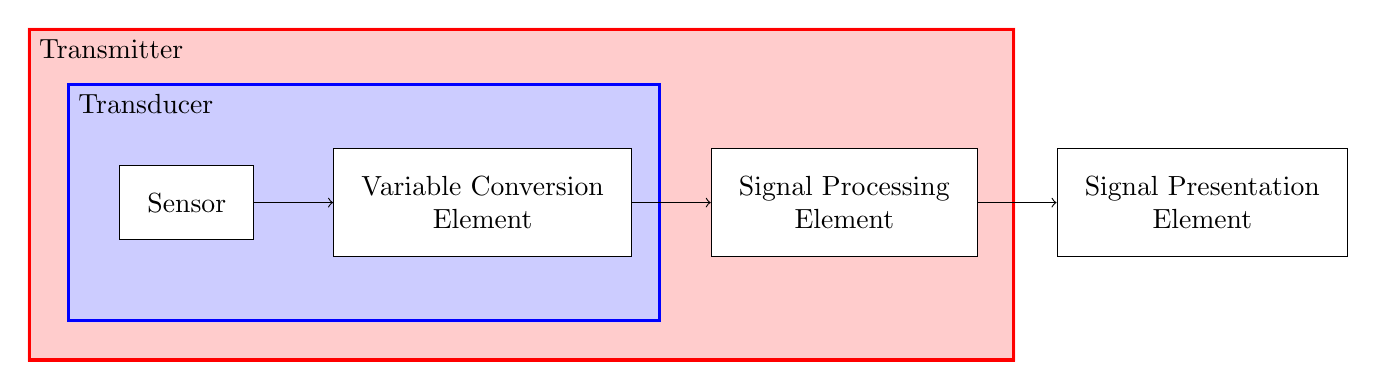
\begin{tikzpicture}[fill=white]
		\begin{scope}[opacity=0.2, transparency group]
			\draw[fill=red, color=red, very thick] (-2,2.2) rectangle (10.5,-2);
			\draw[fill=blue, color=blue, very thick] (-1.5,1.5)  rectangle (6,-1.5);
		\end{scope}
		\draw[color=red, very thick] (-2,2.2) rectangle (10.5,-2);
		\draw[color=blue, very thick] (-1.5,1.5)  rectangle (6,-1.5);

		\node[below right] (a) at (-1.5,1.5) {Transducer};
		\node[below right] (b) at (-2,2.2) {Transmitter};


		\node (sensor) [inner sep=10pt, draw, fill=white] {Sensor};
		\node (vce) [inner sep=10pt, right=of sensor, draw, align=center, fill=white] {Variable Conversion\\Element};
		\node (spe) [inner sep=10pt, right=of vce, draw, align=center, fill=white] {Signal Processing\\Element};
		\node (sppe) [inner sep=10pt, right=of spe, draw, align=center] {Signal Presentation\\Element};
		\draw (sensor) edge[->] (vce);
		\draw (vce) edge[->] (spe);
		\draw (spe) edge[->] (sppe);
	\end{tikzpicture}
\end{figure}

\section{Performance Characteristics}

\begin{itemize}
	\ii Range: The minimum and maximum values of the measurand that can be measured. $[M_{\text{min}}, M_{\text{max}}]$.
	\ii Span: The difference between the maximum and minimum values of the measurand. $M_{\text{max}} - M_{\text{min}}$.
	\ii Full Scale Output: The output of the sensor when the measurand is at its maximum value. $M_{\text{max}}$.
	\ii Rangeability: The ratio of the maximum to minimum values of the measurand that can be measured. $M_{\text{max}} / M_{\text{min}}$.
\end{itemize}

\newpage

\begin{figure}[H]
	\centering
	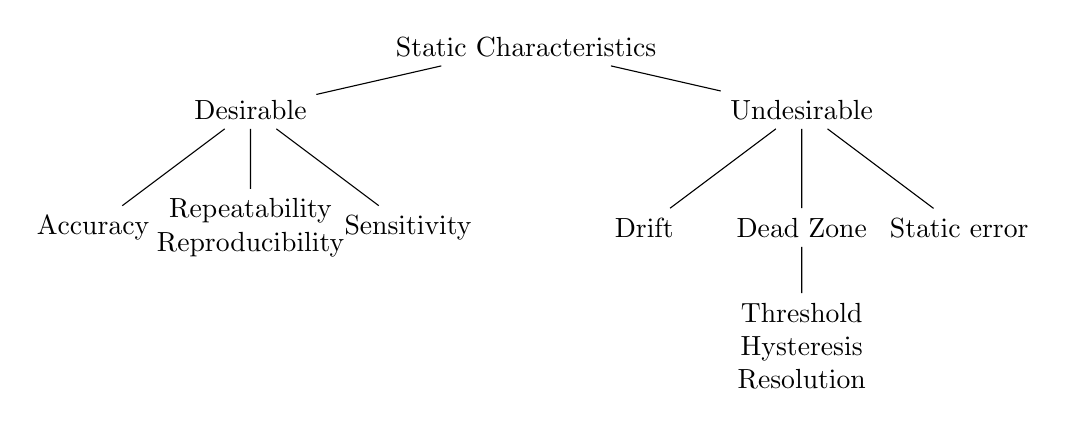
\begin{tikzpicture}[
			level 1/.style = { level distance = 8mm,
					sibling distance = 70mm },
			level 2/.style = { level distance = 15mm,
					sibling distance = 20mm }
		]
		\node {Static Characteristics}
		child {
				node {Desirable}
				% child {node[align=center] {Accuracy\\Sensitivity\\Repeatability\\Reproducibility}}
				child {node {Accuracy}}
				child {node[align=center] {Repeatability\\Reproducibility}}
				child {node {Sensitivity}}
			}
		child {
				node {Undesirable}
				child {node {Drift}}
				child {node {Dead Zone} child {node[align=center] {Threshold\\Hysteresis\\Resolution}}}
				child {node {Static error}}
			};
	\end{tikzpicture}
\end{figure}

\begin{itemize}
	\ii Accuracy: The closeness of the measured value to the true value.
	\ii Sensitivity: The ratio of the change in output to the change in input. $S = \frac{\Delta y}{\Delta x}$. Note that we assume that the relationship between the input and output is linear.
	\ii Repeatability and Reproducibility: The closeness of the output readings when the same input is applied.
	\begin{itemize}
		\ii Precision: The closeness of the output readings when the same input is applied. (Degree of freedom from random error)
	\end{itemize}
\end{itemize}

\begin{figure}[H]
	\centering
	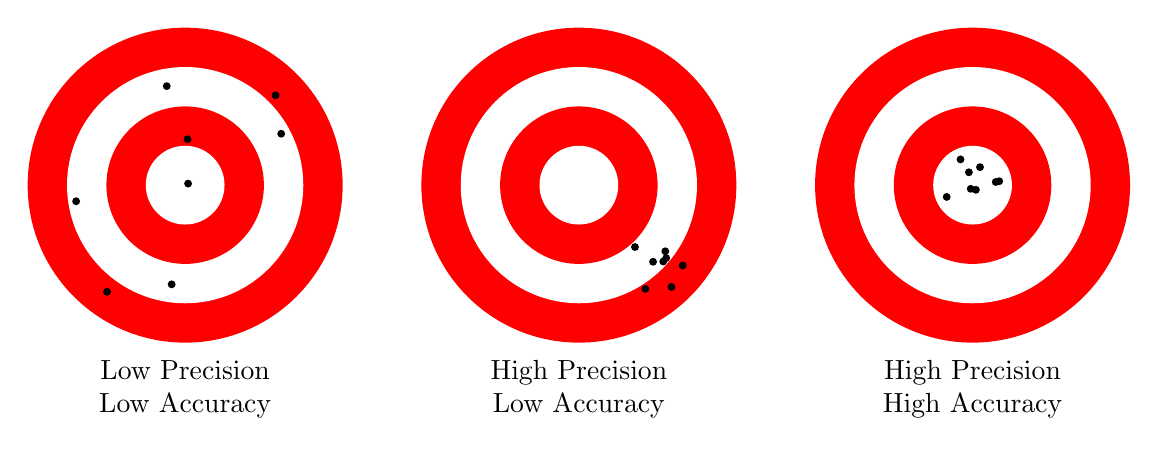
\begin{tikzpicture}
		\begin{scope}
			\fill[red] circle (2);
			\fill[white] circle (1.5);
			\fill[red] circle (1);
			\fill[white] circle (0.5);

			\foreach \i in {1,...,8}
				{
					\fill[black] (rand*1.5,rand*1.5) circle (0.05);
				}

			\node[align=center, below] at (0,-2.1) {Low Precision\\Low Accuracy};
		\end{scope}
		\begin{scope}[xshift=5cm]
			\fill[red] circle (2);
			\fill[white] circle (1.5);
			\fill[red] circle (1);
			\fill[white] circle (0.5);

			\foreach \i in {1,...,8}
				{
					\fill[black] (rand*0.35+1,rand*0.35-1) circle (0.05);
				}

			\node[align=center, below] at (0,-2.1) {High Precision\\Low Accuracy};
		\end{scope}
		\begin{scope}[xshift=10cm]
			\fill[red] circle (2);
			\fill[white] circle (1.5);
			\fill[red] circle (1);
			\fill[white] circle (0.5);

			\foreach \i in {1,...,8}
				{
					\fill[black] (rand*0.35,rand*0.35) circle (0.05);
				}

			\node[align=center, below] at (0,-2.1) {High Precision\\High Accuracy};
		\end{scope}
	\end{tikzpicture}
\end{figure}

\begin{itemize}
	\ii Drift: The change in a static characteristic as a function of ambient conditions.
	\begin{itemize}
		\ii Zero Drift: The change in the output when the input is zero. Usually due to changes in ambient conditions.

		\[
			\text{Zero Drift Coefficient} = \frac{\text{Zero Drift}}{\text{Change in Ambient Conditions}}
			.\]

		\ii Sensitivity Drift: The change in sensitivity as a function of ambient conditions.

		\[
			\text{Sensitivity Drift Coefficient} = \frac{\text{Sensitivity Drift}}{\text{Change in Ambient Conditions}}
			.\]

		\begin{figure}[H]
			\centering
			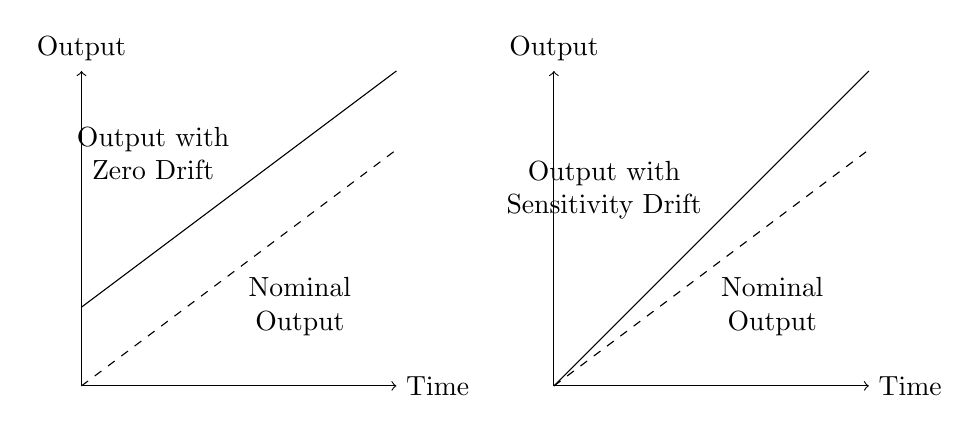
\begin{tikzpicture}
				\begin{scope}
					\draw[->] (0,0) -- (4,0) node[right] {Time};
					\draw[->] (0,0) -- (0,4) node[above] {Output};
					\draw[dashed] (0,0) -- (4,3) node[midway, below right, align=center] {Nominal\\Output};
					\draw (0,1) -- (4,4) node[midway, above left, align=center] {Output with\\Zero Drift};
				\end{scope}
				\begin{scope}[xshift=6cm]
					\draw[->] (0,0) -- (4,0) node[right] {Time};
					\draw[->] (0,0) -- (0,4) node[above] {Output};
					\draw[dashed] (0,0) -- (4,3) node[midway, below right, align=center] {Nominal\\Output};
					\draw (0,0) -- (4,4) node[midway, above left, align=center] {Output with\\Sensitivity Drift};
				\end{scope}
			\end{tikzpicture}
		\end{figure}
	\end{itemize}

	\ii Dead Zone: The range of input values for which the output does not change.

	\begin{itemize}
		\ii Threshold: The minimum input value that causes the output to change.
		\ii Hysteresis: The difference in output when the input is increasing and when it is decreasing.
		\ii Resolution: The smallest change ($\Delta I$) in input that causes a change in output. It can be expressed as a percentage as follows:
		\[
			\frac{\Delta I}{I_{\text{max}} - I_{\text{min}}} \times 100\%
			.\]

		\begin{figure}[H]
			\centering
			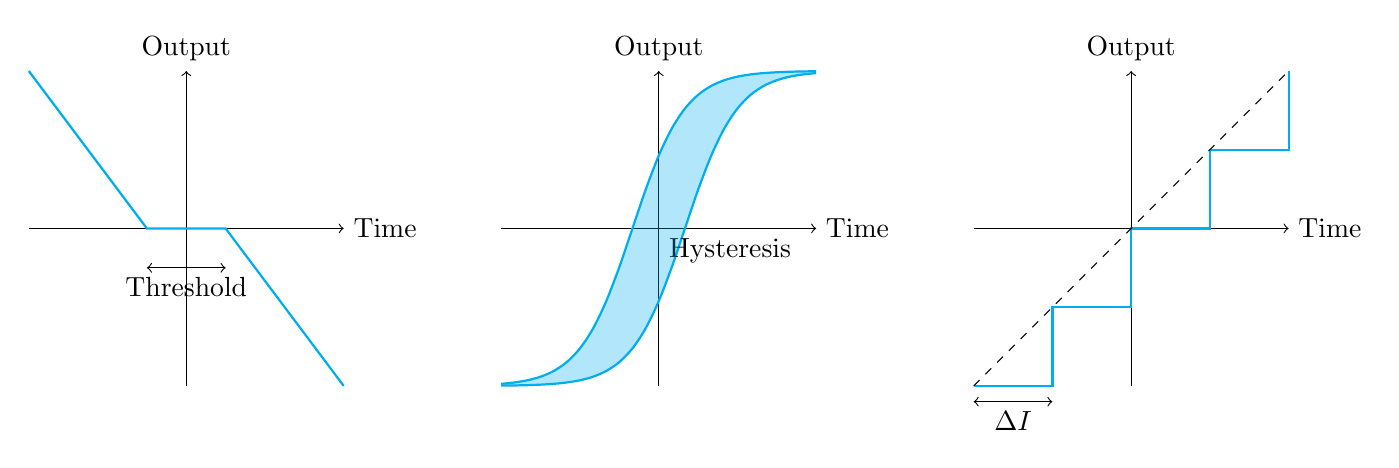
\begin{tikzpicture}
				\begin{scope}
					%threshold
					\draw[->] (-2,0) -- (2,0) node[right] {Time};
					\draw[->] (0,-2) -- (0,2) node[above] {Output};
					\draw[cyan, thick] (-2,2) -- (-0.5,0) -- (0.5,0) -- (2,-2);
					\draw[<->] (-0.5,-0.5) -- (0.5,-0.5) node[midway, below] {Threshold};
				\end{scope}

				\begin{scope}[xshift=6cm]
					\draw[->] (-2,0) -- (2,0) node[right] {Time};
					\draw[->] (0,-2) -- (0,2) node[above] {Output};
					\draw[
						postaction=decorate,
						decoration={mark=at position 0.5 with {\arrow{<}}},
						thick,
						domain=-2:2,
						smooth,
						variable=\x,
						cyan]
					plot ({\x}, {4/(1 + exp(-3*\x+1))-2});
					\draw[
						postaction=decorate,
						decoration={mark=at position 0.5 with {\arrow{>}}},
						thick,
						domain=-2:2,
						smooth,
						variable=\x,
						cyan]
					plot ({\x}, {4/(1 + exp(-3*\x-1))-2}) node[pos=0.75, below right, color=black] {Hysteresis};
					\begin{scope}
						\clip plot[domain=-2:2] ({\x}, {4/(1 + exp(-3*\x+1))-2}) -- plot[domain=2:-2] ({\x}, {4/(1 + exp(-3*\x-1))-2});
						\fill[cyan, opacity=0.3] plot[domain=-2:2] ({\x}, {4/(1 + exp(-3*\x+1))-2}) -- plot[domain=2:-2] ({\x}, {4/(1 + exp(-3*\x-1))-2});
					\end{scope}
				\end{scope}

				\begin{scope}[xshift=12cm]
					% resolution
					\draw[->] (-2,0) -- (2,0) node[right] {Time};
					\draw[->] (0,-2) -- (0,2) node[above] {Output};
					\draw[cyan, thick] (-2,-2) -| (-1,-1) -| (0,0) -| (1,1) -| (2,2);
					\draw[dashed] (-2,-2) -- (2,2);
					\draw[<->] (-2,-2.2) -- (-1,-2.2) node[midway, below] {$\Delta I$};
				\end{scope}
			\end{tikzpicture}
		\end{figure}
	\end{itemize}
\end{itemize}

\section{Dynamic Characteristics}

The dynamic characteristics of an instrumentation system are the characteristics that describe the system's response to a change in the measurand. The response to an input value can be:

\begin{itemize}
	\ii Zero Order: The output is constant until the input changes. $O= kI$
	\ii First Order: The output changes similarly to a first order differential equation. $O = k(1 - e^{-t/\tau})$
	\ii Second Order: The output changes similarly to a second order differential equation.
\end{itemize}

\begin{figure}[H]
	\centering
	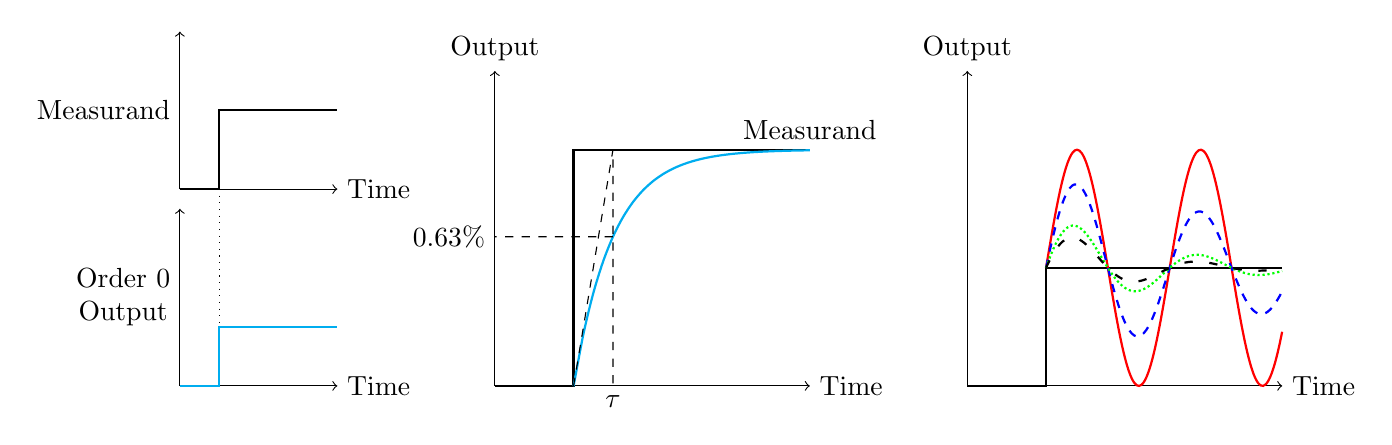
\begin{tikzpicture}
		\begin{scope}[yshift=2.5cm]
			\draw[->] (0,0) -- (2,0) node[right] {Time};
			\draw[->] (0,0) -- (0,2) node[midway, left] {Measurand};
			\draw[thick] (0,0) -- (0.5,0) |- (2,1);

			\draw[->] (0,-2.5) -- (2,-2.5) node[right] {Time};
			\draw[->] (0,-2.5) -- (0,-0.25) node[midway, left,align=center] {Order 0\\Output};
			\draw[cyan, thick] (0,-2.5) -- (0.5,-2.5) |- (2,-1.75);

			\draw [dotted] (0.5,0) -- (0.5,-1.75);
		\end{scope}
		\begin{scope}[xshift=4cm]
			\draw[->] (0,0) -- (4,0) node[right] {Time};
			\draw[->] (0,0) -- (0,4) node[above] {Output};

			\draw[thick] (0,0) -- (1,0) |- (4,3) node[above] {Measurand};
			\draw[
				thick,
				domain=1:4,
				smooth,
				variable=\x,
				cyan]
			plot ({\x}, {3-exp(-(\x-1.55)/0.5)});
			\draw[dashed] (1,0) -- (1.5,3) -- (1.5,0) node[below] {$\tau$} (1.5,1.894) -- (0,1.894) node[left] {$0.63\%$};
		\end{scope}
		\begin{scope}[xshift=10cm]
			\draw[->] (0,0) -- (4,0) node[right] {Time};
			\draw[->] (0,0) -- (0,4) node[above] {Output};

			\draw[thick] (0,0) -- (1,0) |- (4,1.5);

			\foreach \i/\color/\style in {0/red/solid, 0.25/blue/dashed, 0.75/green/densely dotted, 1/black/loosely dashed} {
					\draw[
						thick,
						domain=1:4,
						smooth,
						variable=\x,
						color=\color,
						samples=100,
						\style]
					plot ({\x}, {1.5*exp(-\i*\x) * sin(deg(4*\x-4))+1.5});
				}
		\end{scope}
	\end{tikzpicture}
\end{figure}

\section{Instrument Types}

Instruments can be divided into separate classes according to several properties:

\begin{itemize}
	\ii Active and Passive Instruments: Active instruments require an external power source to operate, while passive instruments do not.
	\ii Null and Deflection Instruments: Null instruments are instruments that measure the measurand by exterting an opposing force to the measured quantity, while deflection instruments measure the measurand by measuring the force exerted bu the measured quantity.
	\ii Analog and Digital Instruments: Analog instruments display the measurand as a continuous value, while digital instruments display the measurand as a discrete value.
	\ii Smart Instruments: Instruments that incorporate a microprocessor to perform signal processing and communication.
\end{itemize}

\chapter{Errors in Instrumentation}

Measurement error is the difference between the measured value and the true value of the measurand. Let $X$ be the true value of the measurand, and $Y$ be the measured value. The error can be expressed as follows:

\begin{itemize}
	\ii Absolute Error: $e_0 = \abs{Y - X}$
	\ii Relative Error: $e_r = \frac{e_0}{X}$
	\ii Percentage Error: $\% e_0 = e_r \times 100\%$
	\ii $X \approx Y (1\pm e_r)$
	\ii Relative error: $A = 1-e_r$
\end{itemize}

The sources of error in instrumentation can be categorized as follows:

\begin{itemize}
	\ii Gross Errors: Errors that are caused by human mistakes. It is not subject to statistical analysis.
	\ii Systematic Errors: Errors that are caused by a constant bias in the measurement. It is caused by two major sources:
	\begin{itemize}
		\ii Instrumental Errors: that are caused by mis-callibration, disturbances caused by the act of measurement, or aging of the instrument.
		\ii Environmental Errors: Errors that are caused by changes in the environment quantified by sensitivity drift and zero drift.
	\end{itemize}
	\ii Random Errors: Errors that are caused by random noise in the measurement. These errors can be modeled using a statistical analysis.
\end{itemize}

\section{Statistical Analysis}

The arithmetic mean of a set of measurements is given by:

\[
	\bar{x} = \frac{1}{n} \sum_{i=1}^{n} x_i
	.\]

The median is the middle value of the set of measurements when they are arranged in ascending order.

\[
	\tilde{x} = \begin{cases}
		x_{\frac{n+1}{2}}                                 & \text{if $n$ is odd}  \\
		\frac{1}{2} (x_{\frac{n}{2}} + x_{\frac{n}{2}+1}) & \text{if $n$ is even}
	\end{cases}
	.\]

The variance of a set of measurements is given by:

\[
	V = \sigma^2 = \frac{1}{n-1} \sum_{i=1}^{n} (x_i - \bar{x})^2
	.\]

The standard deviation is the square root of the variance. $\sigma = \sqrt{V}$.\\

Usually, measurement errors are assumed to be normally distributed. The error limita for a confidence level of the boundaries $c$:

\[
	\pm e = \pm c \lt( \frac{\sigma }{\sqrt{n}} + \sigma \rt) \rightarrow x = y \pm e
	.\]

\section{Aggregate Error}

The aggregate error is the error that is caused by the combination of systematic and random errors. The aggregate error can be expressed as the sum of the systematic and random errors: $\pm e = \pm(e_\text{systematic} + e_\text{random})$.
The \emph{most probable error} (which is a better estimate of the error) can be expressed as follows:

\[
	\pm e = \pm \sqrt{{e_\text{systematic}}^2 + {e_\text{random}}^2}
	.\]

Aggregate errors from separate measurements:

\begin{itemize}
	\ii Error in a sum and difference in terms of given absolute errors:
	\begin{itemize}
		\ii Boundaries error: $\pm e = \pm (y_1e_{r_1} + y_2e_{r_2})$
		\ii Most probable error: $\pm e = \pm \sqrt{{e_{r_1}}^2 + {e_{r_2}}^2}$
		\begin{align*}
			x_1 + x_2 & = (y_1 + y_2) \pm e_0 = (y_1 + y_2)(1\pm e_r) = (y_1 + y_2) \pm \% e_0 \qq{with} e_r = \frac{e_0}{y_1+y_2} \qand \% e_0 = e_r \times 100 \\
			x_1 - x_2 & = (y_1 - y_2) \pm e_0 = (y_1 - y_2)(1\pm e_r) = (y_1 - y_2) \pm \% e_0 \qq{with} e_r = \frac{e_0}{y_1-y_2} \qand \% e_0 = e_r \times 100
		\end{align*}
	\end{itemize}

	\ii Error in a product and quotient in terms of given absolute errors:
	\begin{itemize}
		\ii Boundaries error: $\pm e_r = \pm (e_{r_1} + e_{r_2})$
		\ii Most probable error: $\pm e_r = \pm \sqrt{{e_{r_1}}^2 + {e_{r_2}}^2}$

		\begin{align*}
			x_1x_2          & = y_1y_2(1\pm e_r) = y_1y_2 \pm \% e_0 \qq{with} e_r = \frac{e_0}{y_1y_2} \qand \% e_0 = e_r \times 100                    \\
			\frac{x_1}{x_2} & = \frac{y_1}{y_2}(1\pm e_r) = \frac{y_1}{y_2} \pm \% e_0 \qq{with} e_r = \frac{e_0}{y_1/y_2} \qand \% e_0 = e_r \times 100
		\end{align*}
	\end{itemize}
\end{itemize}

\end{document}
